\documentclass[a4paper, 12pt,oneside]{article} 
%\documentclass[a4paper, 12pt,oneside,draft]{article} 

\usepackage{preamble}
\usepackage{bm}
% structure check 
% confounding factor 
% computations (with )
%--------------------- ACTUAL FILE ---------------------- %
\begin{document} 
	\begin{center}
	    \Large
	    \textbf{Project 7 : Request from a Clinical Dietitian}
	    \vspace{0.4cm}
	    \large
        
	    Author : Tara Fjellman \\
	    \small{Spring 2024}
	\end{center}
	\section{Introduction}
	The purpose of this report is to help a clinical dietitian do a power analysis for a study. The goal of the study is to compare two different diets, $A$ and $B$, for diabetic patients. We take a statistical consulting approach to propose a solution, making sure the explanations are clear so that the dietitian can understand the results. We also provide a few ideas to improve the study's design.
    \section{Request analysis}
	\subsection{Understanding the request}
	From what I understand the clinical dietitian wants to compare the two diets for diabetic patients and plans to proceed as follows : (a) create two equally sized groups of subjects by randomly selecting diabetic patients from a database and randomly assigning them to one of the two diets; (b) have each of the patients follow their associated diet for a duration of six weeks; (c) conduct a fasting blood glucose test on each patient.

	She hypothesizes that diet $A$ will be better than $B$, leading to on average around 10 mg/dl lower blood glucose. Given this, she wants to know how many subjects are needed in each group. 
	\subsection{Clarifications}
	Given what is mentioned in the previous section, I would have a few questions to clarify the problem :
	\begin{enumerate}
		\item What type of diabetes are we considering ? Type I, Type II, or both ? This is important as the two types of diabetes might respond differently to treatments. If we are considering both types, this should be accounted for in the analysis. 
		\item Are the measurements guaranteed to all be taken within the same conditions ? Could there be any sources of systematic error ? (for example : Will the used apparatus be the same ? Will the tests be taken on the same day ?). It is important to make sure the measurements are taken under the same conditions to ensure they are comparable and that the systematic errors are not deteriorating the quality of the data (eg. affecting the independence of the data, see next section for a definition of independence). 
		\item After some research, I found that the standard deviation of blood glucose is typically around 15 mg/dl. Does this correspond to your expectations ? Do you have any reasons to believe that it is likely for the standard deviation to be different in one of the groups ? (eg. could the effect of any products included in the diets could be really subject-dependent ?). This is important as it may highly affect the number of subjects needed for the study. The same questions for the given estimate of the effect size ($10$ mg/dl) is also relevant.
		\item Additionally, I would like to know if you have any previous data on the subject. This could help us determine the number of subjects needed. The contact of the statisticians that have helped you in the past could also be useful. This could help us understand the problem better and leverage prior work.
	\end{enumerate}
	In the bulk of the analysis I assume that you are considering one single type of diabetes, that the measurements are taken under sufficiently similar conditions and, that the standard deviations of the blood glucose are in the 12 to 18 mg/dl range (allowing for different situations).
	%I later address ways in which we could improve the analysis if the assumptions are not met.
	\subsection{Formal prerequisites}
	To understand the problem and propose a quantitative solution, some formal statistical concepts are needed. The goal of this section is to introduce them in simple terms.

	Firstly, we need to introduce the concept of statistical independence (also just called independence). Two events are independent if the occurrence of one does not affect the occurrence of the other. For example, if we flip coin twice, the outcome of the first flip does not affect the outcome of the second flip. This concept is important in this context as we want to make sure that the measurements associated to different individuals are independent.

	Another concept which we will need is that of a gaussian distribution. For our purpose, we can understand it as the description of a process in terms of its typical value (called its mean) and its typical fluctuation from this value (called its standard deviation). An example of such process is the height of adults in a given country. In this case the mean would be around 170 cm and the standard deviation around 10 cm. Indeed when asking a random adult about their height, we would expect them to be around 170 cm tall, but we would not be surprised if they were 10 cm taller or shorter. This concept will be used to model the average blood sugar associated to each of the groups. 

	We also need to introduce the concept of confounding variables (also called confounders). A confounder is a hidden factor that affects both the cause and effect of what you are studying. It makes it hard to tell if the cause really leads to the effect. For example, if we want to study the effect of a new drug on a disease, but we do not control for the age of the patients, we might falsely attribute the effect of the age to the drug. Saying that there are no confounders can be understood as saying that we have access to all the relevant variables. This is important in this context as we want to make sure that the dietitian's hypothesis is not affected by other factors.

	The last important concept we need to introduce is that of a two-sample hypothesis test. Such a test is a statistical computation that is used to determine weather two observations come from the same process. For example, we could use such a test to check whether the mean height of adults in two countries differs from one sample of people from each country. Given the observations $Y_A,Y_B$ of country $A$ and $B$, we would then compare two models : (a) there is no difference (we call this the null model); (b) the first population is on average taller (we call this the alternative model). In statistics, to be precise about "whether the mean height of adults in two countries differs" we use the concepts of statistical significance and power. Statistical significance is the probability of an observation at least as drastic as the one made when assuming the null model holds. In our case it would be the probability for the $Y_A-Y_B$ difference to be at least as large as the one observed assuming that the two populations have the same mean height. If this probability is smaller than $\alpha$ (often taken as 0.05), we can say that the observation is statistically significant at level $\alpha$. The power of a test is defined in analogy but this time assuming the alternative model holds. We often require this probability to be higher than 0.8. Statistical power is often denoted $1-\beta$.
	These concepts will be important to formalise the test the dietitian wants to run : diet $A$ is better than diet $B$. Here the null model is that the two diets have the same effect on the blood glucose levels, while the alternative model is that diet $A$ is better. 
	\section{Candidate solution}
	As a solution for this initial stage of the study we make use of a two sample z-test to compare the means of the two groups.
	This encompasses making two assumptions : (1) the means of the two groups are gaussianly distributed (reasonable for large enough groups by the central limit theorem if the measurements are independent); (2) we know the standard deviations of the two groups, say $\sigma_A$ and $\sigma_B$. This second assumption is in reality not satisfied currently as we only have a rough idea that the standard deviation of blood glucose will be around 15 mg/dl. In practice, one can avoid making this assumption by using a slightly more complicated test (a Welch t-test), but this requires the experimental data to be available (which is not yet the case). As we do not have access to the data yet, we will assume that we know the standard deviations and make up for this by considering different values for them. For simplicity we fix $\sigma_B$ and make $\sigma_A$ vary. 
	\subsection{Procedure explanation}
	Given values for the effect size $\Delta \mu$, and the two standard deviations $\sigma_A,\sigma_B$, we define the test statistic as $T=\overline{Y}_A-\overline{Y}_B$ where $\overline{Y}_A,\overline{Y}_B$ respectively are the average blood sugar levels associated to diet $A$ and $B$. Under the null model, the two means are equal and the test statistic is gaussianly distributed with mean $0$ and standard deviation $\sigma_{T}=\sqrt{\frac{\sigma_A^2}{n}+\frac{\sigma_B^2}{n}}$. Under the alternative model, the test statistic has this same standard deviation but a mean of $\Delta \mu$.

	With this in mind, we can compute the critical threshold $t_{1-\alpha}$ by imposing that (under the null) the probability of observing a value at least as extreme as the observed one is $\alpha$ and solving for $T$ :
	$$
	\text{Pr}(T\geq t_{1-\alpha}\mid \mu=0, \sigma=\sigma_{T})\overset{!}{=}\alpha
	%1-\text{Pr}(T\leq t_{\alpha})=
	\iff 1-\Phi(t_{\alpha};\mu=0, \sigma=\sigma_{T})\overset{!}{=}\alpha.
	$$
	Once this is done, we can compute the power of the test by imposing that (under the alternative) the probability of observing a value at least as extreme as the observed one is $1-\beta$ :
	$$
	\text{Pr}(T\geq t_{1-\alpha}\mid \mu=\Delta\mu, \sigma=\sigma_{T})\overset{!}{=}1-\beta
	%1-\text{Pr}(T\leq t_{\alpha})=
	\iff 1-\Phi(t_{\alpha};\mu=\Delta\mu, \sigma=\sigma_{T})\overset{!}{=}1-\beta.
	$$
	In the following we take $\alpha=0.05$ and $1-\beta=0.8$, as we found by doing some research online that dietitians usually do so.
	Applying this procedure for a range of values of the group size $n$, we can determine the minimal group size needed to achieve the wanted power level. An example of this for $\Delta\mu=10$ mg/dl and $\sigma_A=\sigma_B=15$ mg/dl is shown in \ref{fig:power-vs-group-size}.	
	\begin{figure}[h!]
		\centering
		\vspace{0em}
		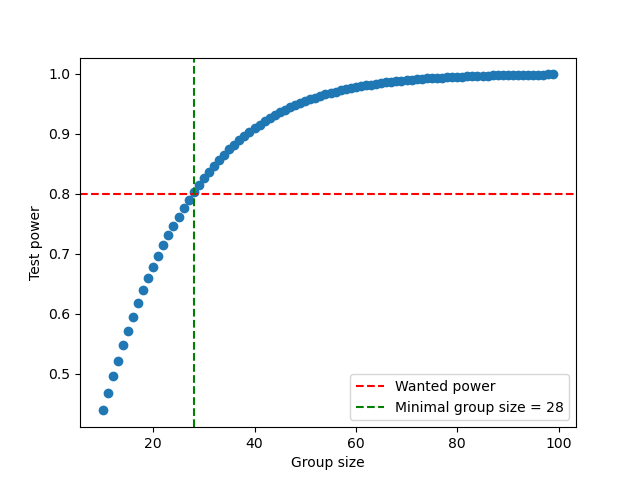
\includegraphics[width=.7\textwidth]{power-vs-group-size}
		\caption{Test power (at significance level 0.05) as a function of the group size. The red and green lines respectively represent the power level of $80\%$ and the minimal group size for which we have this power. In this case $\Delta \mu=10$ mg/dl and $\sigma_A=\sigma_B=15$ mg/dl.}
		\label{fig:power-vs-group-size}
	\end{figure}
	Looking at the figure we see that the minimal group size needed to achieve a power level of $80\%$ is of $28$ subjects. We also see that one can clearly reach higher test power by increasing the group size, but that this increase saturates fast after the selected one. This is a typical feature of power curves. 
	\subsection{Mean and standard deviation variation}
	As mentioned, we do not have access to the data yet and thus do not know the exact values of the standard deviations. In this section we therefore consider different values for them to see how the minimal group size is affected. The results of the simulations are shown in \ref{fig:minimal-group-size-simulations} by making both the effect and the standard deviation of the treated group vary by 20\% around the default values of $\Delta\mu = 10$ mg/dl, $\sigma_A=15$ mg/dl. 
	\begin{figure}[h!]
		\centering
		\vspace{0em}
		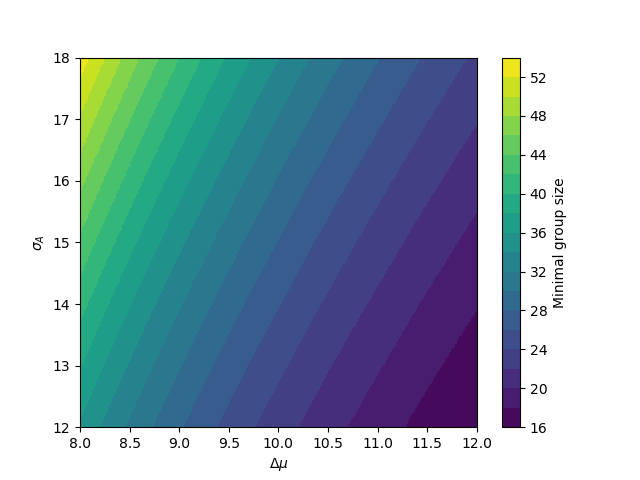
\includegraphics[width=.7\textwidth]{minimal-group-size-simulations}
		\caption{Minimal group size associated to the wanted power (at significance level 0.05) as a function of the effect size and the standard deviation of the $A$ group. The standard deviation of the 
		$B$ group is taken as $\sigma_B=15$ mg/dl.}
		\label{fig:minimal-group-size-simulations}
	\end{figure}
	We see that the minimal group size needed to achieve the wanted power level increases with a standard deviation increase and decreases with a effect size increase. This is expected as the two groups are harder to distinguish whenever the distributions of their means overlap and : larger standard deviations increase this overlap, while larger effect sizes decrease it.
	Notice that the increase is steepest as a function of standard deviation when the effect size is small (for this same reason).
	To better understand this effect, we can look at a couple different scenarios represented in \ref{fig:scenarios}.
	\begin{figure}[h!]
		\centering
		\vspace{0em}
		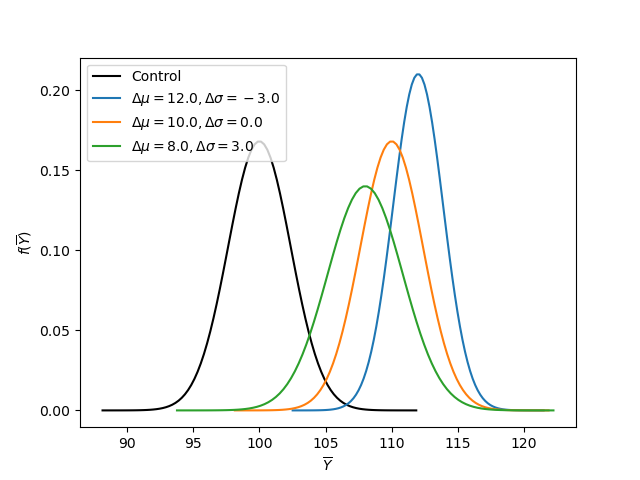
\includegraphics[width=.7\textwidth]{scenarios}
		\caption{Distributions of the average blood sugar levels for the $B$ group and some possible $A$ groups with different effect size and standard deviation. Here the group size is taken as $n=40$.}
		\label{fig:scenarios}
	\end{figure}
	Looking at the figure we indeed see that the scenarios corresponding to larger overlap between the control and trial distributions of average blood sugar levels require larger group sizes to achieve the wanted power level. 

	Analysing now \ref{fig:minimal-group-size-simulations} further, we see that the minimal group size needed varies largely with the effect size and the standard deviation. This number goes from 16 to 53 between the two most extreme scenaries ($\Delta\mu=12\text{ mg/dl},\sigma_A=12\text{ mg/dl}$ vs. $\Delta\mu=8\text{ mg/dl},\sigma_A=18\text{ mg/dl}$). It is therefore really important to have a grasp of the range of possible values for these two parameters to determine the minimal group size needed. For example, if want to accommodate for an effect size as small as 9.0 mg/dl and a standard deviation as large as 16.5 mg/dl, we should consider a group size of minimum 38 subjects. 
	\section{Possible improvements}
	In this section we propose a few ways in which the analysis could be improved.
	\subsection{Avoid confounding variables}
	As mentioned, a confounding variable is a hidden factor that affects both the cause and effect you are studying. It makes it hard to tell if the cause really leads to the effect. The random assignment of the patients to the two groups should help us avoid this issue. However, if the two groups are not comparable in terms of all relevant variables, the results of the study could be biased. There are a couple of ways in which we could improve this. 

	The most thorough solution is to consider a single group and measure the blood sugar levels twice : once before the six week diet; and once after. Then, one can consider the average difference obtained by comparing for each subject the two measurements. This allows to control for all the variables that could affect the blood sugar as long as the subjects do not vary their lifestyle too much during the six weeks of dieting. This would however require the subjects to be tested on two different days, which might be impractical. To avoid other sources of confounding variables we should then also make sure that the tests are taken under the same conditions on both days.

	A similar solution, but that does not require two tests per subject, consists in matching subjects smartly. Indeed, if you know which variables could affect the blood glucose levels, we could create the two groups by paring subjects who share the same characteristics. For example, if we know that age and sex of patients affects the blood glucose levels, we should make sure that the two groups have the same age and sex distribution. Then, we would proceed as before, by comparing the average difference in blood glucose levels between the created pairs. This method would however require a good understanding of the variables that affect the blood glucose levels.

	Both of these solutions could also serve as ways to reduce the observed variance.
	\subsection{Use more of the data}
	Another way in which we could improve the analysis' power and reach is by using more data associated to the subjects. We could for example take advantage of the created groups to study the effects of the diets on symptoms other than blood glucose levels (as thirst, polyuria, weight loss, and blurred vision). This would allow us to get a more complete picture of the effects of the diet. This could be done by measuring the levels of other compounds in the blood, or by asking the subjects to fill out a questionnaire. 

	This could also allow to start and get an idea for what the secondary effects of the diet are (if there are any).

	This change would require the analysis to account for the multiple testing.
	%\subsection{Avoid assuming std knowledge}
	\section{Conclusion}
	In this report we have proposed a solution to the dietitian's request, and made it accessible for her to understand. We have shown that the minimal group size needed to achieve a power level of $80\%$ (at significance level $0.05$) is around $38$ subjects. This result was however found to vary largely in terms of the exact effect size and the standard deviation of the treated group, putting emphasis on the importance of a good range estimate for these parameters. Some key clarification questions that could affect the analysis were brough up and a few improvements on the current design proposed. I am looking forward to following up on this analysis with you and helping you with the next steps of the study.
	%\section*{References}
\end{document}